%!TEX root = ../summary.tex

\section{Software Architectures and their Trade-Offs}

\subsection{Introduction to Distributed Systems and Middleware}
Distributed systems are physically disjoint compute resources interconnected by a network.
They are characterized by reliability, availability, heterogeneity, openness (for extension), security, scalability, fault tolerance and failure handling, concurrency, transparency and predictable performance.\\
A middleware provides services and abstractions to facilitate design, development and deployment of distributed applications in heterogeneous, networked applications.

\subsection{Database-Centric Architectures}
The main purpose of database-centric architectures is data access and updates.
Thereby the traditional, passive approach only responds to requests whereas in a backboard or active system clients solve problems collaboratively and the system updated the clients whenever information changes.
These architectures favor stored procedures running on database servers over middle-tier application servers.\\

The classical \textbf{mainframe model} uses one central computer/repository for information and clients are just terminals that connect to it.\\
\begin{minipage}[t]{0.49\textwidth}
    \textbf{Pros}
    \begin{itemize}[topsep=0pt,noitemsep]
        \item Hardware maintenance cost reduction
        \item Single point of administration
        \item One type of administrative skill set
        \item Simple architecture and low bandwidth requirements
    \end{itemize}
\end{minipage}
\begin{minipage}[t]{0.49\textwidth}
    \textbf{Cons}
    \begin{itemize}[topsep=0pt, noitemsep]
      \item Single point of failure
      \item Character-based applications
      \item Bottlenecks due to time-sharing systems
    \end{itemize}
\end{minipage}
\vspace{20pt}

The \textbf{three-layered client/server architecture} consists of a client, a web server and data sources.\\
\begin{minipage}[t]{0.49\textwidth}
    \textbf{Pros}
    \begin{itemize}[topsep=0pt,noitemsep]
      \item Reduced hardware costs
      \item No single point of failure
      \item Flexibility
      \item Scalable architecture
    \end{itemize}
\end{minipage}
\begin{minipage}[t]{0.49\textwidth}
    \textbf{Cons}
    \begin{itemize}[topsep=0pt, noitemsep]
      \item Heightened administrative costs
      \item Increased security risks
      \item Lack of centralized backup
    \end{itemize}
\end{minipage}
\vspace{20pt}

Databases have base relations which correspond to the entities in the conceptual schema.
\textbf{Views} then are the dynamic result of one or more relational operations on a database that produce another relation that does not physically exist in a database but is created upon request.\\
\begin{minipage}[t]{0.49\textwidth}
    \textbf{Pros}
    \begin{itemize}[topsep=0pt,noitemsep]
      \item Data independence
      \item Improved security
      \item Reduced complexity
      \item Convenience
      \item Customization
      \item Data integrity
    \end{itemize}
\end{minipage}
\begin{minipage}[t]{0.49\textwidth}
    \textbf{Cons}
    \begin{itemize}[topsep=0pt, noitemsep]
      \item Update restriction
      \item Structure restriction
      \item Performance
    \end{itemize}
\end{minipage}
\vspace{20pt}

It is also possible to store subprograms which are PL/SQL blocks that take parameters and can be invoked.
It can be differentiated between \textbf{(stored) procedures} and functions where functions always return values and procedures not.
By processing SQL code on the database server, the number of instructions and the amount of data returned are reduced.
A package in this context is defined as a collection of procedures, functions, variables and SQL statements in a single program unit.\\
\begin{minipage}[t]{0.49\textwidth}
    \textbf{Pros}
    \begin{itemize}[topsep=0pt,noitemsep]
      \item Extensibility
      \item Reusability
      \item Maintainability
      \item Aid abstraction
      \item Improves testability (Can be tested independently of the application)
      \item Speed / optimization (Stored procedures are cached on the server)
      \item Improved security
    \end{itemize}
\end{minipage}
\begin{minipage}[t]{0.49\textwidth}
    \textbf{Cons}
    \begin{itemize}[topsep=0pt, noitemsep]
      \item Limited Coding Functionality
      \item Portability issues
      \item Testing (Any data errors in handling stored procedures are not generated until runtime)
      \item Reduced flexibility and agility
    \end{itemize}
\end{minipage}
\vspace{20pt}

\subsubsection{Data Warehousing and Business Intelligence}
Business intelligence is the extraction of knowledge from large amounts of business data using a variety of technologies like data warehousing, data mining and others.
Data warehousing is a collection of methods, techniques and tools which is used to support knowledge workers like senior managers and directors to conduct data analyses that help with performing decisions and improving information resources.\\
Usually the initial situation is that data is given in a heterogeneous, erroneous state.
Therefore it has to be transformed to be stored in the central data warehouse using a process called on-line transformation processing (OLTP).
For this ``extract, transform, load (ETL)'' is applied, where first the data is extracted from previous data stores, then transformed and cleansed and finally loaded into the DW\@.
So called data marts can then used to get subsets of the stored data that is relevant to specific business areas or users.
This part of data warehousing is called on-line analytical processing (OLAP).
The structure of DW is shown in Figure~\ref{fig:data_warehousing}.\\
\begin{figure}[h]
  \centering
  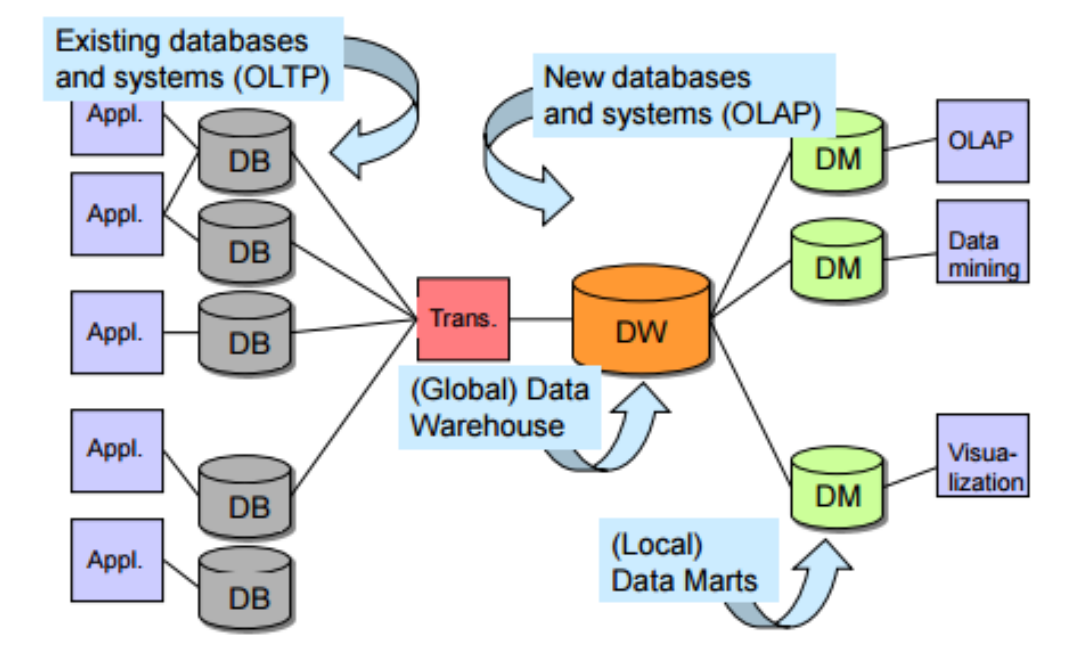
\includegraphics[width=.8\textwidth]{images/data_warehousing.png}
  \caption{Data Warehousing Structure}\label{fig:data_warehousing}
\end{figure}

DWs can have different structures.
One options is a \textbf{central DW} where all data is stored in one point.
This approach is very simple to manage but has bad performance due to the massive workload at that point.\\
A second variety is to have \textbf{multiple data marts} which are aimed at specific departments and store corresponding data.
The DW only exists logically.
This approach increases performance due to the distributed workload but is more complex.\\
The most complex but also most performant approach is to have a central warehouse where data is distributed to \textbf{data marts on multiple tiers}.
When querying, data is aggregated and reduced as it moves through tiers.\\

Data warehousing is a good approach to handle large amounts of data.
As always, it does not only have advantages though.
DW projects are usually very costly in time (12 - 36 month) and money (1 million US\$ or more).
Furthermore no design methodologies, insufficient training and some ethical considerations (security, privacy) exist.

\subsubsection{Big Data Architectures}
Big data is high-volume, high-velocity and high-variety information assets that demand cost-effective, innovative forms of information processing for enhanced insight and decision making.

\paragraph{Scalability}
Scalability is one of the key concepts of big data.
It refers to the ability of a system to handle a growing amount of work in a capable manner or its ability to be enlarged to accommodate that growth. We differentiate between vertical and horizontal scaling.\\
In \textbf{vertical scaling} an existing IT resource is replaced with another one with higher or lower capacity.
If an replacement with an resource of lower capacity takes place, we speak of scaling up whereas an replacement with a higher capacity one is called scaling down.
The advantage of this approach is that it is very easy to design vertical scaling.\\
When \textbf{scaling horizontally} resources are allocated or released dynamically.
Resource allocation is called scaling out and resource releasing is called scaling in.
This approach is usually cheaper in the long run.\\

In horizontal scaling, data is divided across so called \textbf{shards}.
Every shard hold the same schemas, but its own subsets of the data.
Every shard can be placed on a separate node what spreads the read and write operations across the cluster.
When trying to query this distributed database then, different strategies how to look for specific data can be applied.\\
The \textbf{lookup strategy} maintains a lookup table in a central node and forwards queries to the according shard based on a shard key and that table.\\
The \textbf{range strategy} stores ranges of data on shards in sequential order. This can be used to determine which shard particular data is stored on.\\
Lastly the \textbf{hash strategy} calculates hashes of keys and distributes data based on that hash.
This has the advantage that data is less clustered which implies better load balancing.\\

\paragraph{NoSQL Data Stores}
Next generation databases mostly addressing some of the points: being non- relational, distributed, open-source and horizontally scalable.\\

\textbf{Key-value stores} store data in an unstructured way by storing a key and an associated value.
This approach usually has quite poor performance in cases that require processing of key ranges.
This might be overcome with ordered key-value approaches.
Value modeling is not included in this approach.\\
\begin{minipage}[t]{0.49\textwidth}
  \textbf{Pros (Redis)}
  \begin{itemize}[topsep=0pt,noitemsep]
    \item Disk-backed, in-memory database
    \item Master-slave replication, automatic failover
    \item Support for multiple data types
    \item Lua scripting capabilities
    \item Transaction support
    \item Values can be set to expire
    \item Pub/sub to implement messaging
  \end{itemize}
\end{minipage}
\begin{minipage}[t]{0.49\textwidth}
  \textbf{Cons (Redis)}
  \begin{itemize}[topsep=0pt, noitemsep]
    \item Dataset size limited to computer RAM (but can span multiple machines' RAM with clustering)
    \item Not suitable for complex applications with complex data models
    \item Not suited for interconnected (graph) data
    \item As the volume of data increases maintaining unique keys becomes more difficult and requires some complexity in generating character strings that will remain unique over a large set of keys
  \end{itemize}
\end{minipage}
\vspace{20pt}

\textbf{Bigtable} is a distributed storage system for managing structured data and is designed to scale to very large sizes.
It maps two arbitrary string values (row and column key) and a timestamp to an arbitrary byte array.
Columns are sorted e lexicographically and are divided into so called tablets for load distribution.
Columns have names of the form $family:qualifier$ and timestamps are used to version the data.\\
\begin{minipage}[t]{0.49\textwidth}
  \textbf{Pros}
  \begin{itemize}[topsep=0pt,noitemsep]
    \item Performance of queries in petabytes of data
    \item Scalability by adding horizontally systems
    \item Availability across the globe
    \item Flexibility since no standard is defined
    \item High speed retrieval independent of location
    \item Data reliability even when disks fail
    \item Storage size by harnessing the power of cheap disks
    \item Versioning of data
  \end{itemize}
\end{minipage}
\begin{minipage}[t]{0.49\textwidth}
  \textbf{Cons}
  \begin{itemize}[topsep=0pt, noitemsep]
    \item No support for (RDBMS-style) multi-row transactions
    \item Offers no consistency guarantees for multi-row updates or cross-table updates (not even eventually)
    \item Lacks the freeform nature of json documents
    \item No join functionality
  \end{itemize}
\end{minipage}
\vspace{20pt}

\textbf{Document-oriented databases} store data based on documents.
No database scheme has to be set up which enables fast, agile development.
Everything concerning an object is encapsulated together which increases performance since data can be read sequentially.
An example for such a database is MongoDB\@.
A sharded cluster in Mongo consits of shards, query routers (mongos) and config servers.
Mongos distribute querys according to the configs in the config servers to the shard holding the matching data.\\

\textbf{Graph databases} store connections as first class citizens, readily available for any “join-like” navigation operation. Accessing those already persistent connections is an efficient, constant-time operation and allows you to quickly traverse millions of connections per second per core.\\
\begin{minipage}[t]{0.49\textwidth}
  \textbf{Pros}
  \begin{itemize}[topsep=0pt,noitemsep]
    \item Fast runtime queries
    \item Constant time traversals in depth and breadth
    \item Shortcuts possible by inserting new transitions
    \item compact storage and memory caching and thus efficient scaling
  \end{itemize}
\end{minipage}
\begin{minipage}[t]{0.49\textwidth}
  \textbf{Cons}
  \begin{itemize}[topsep=0pt, noitemsep]
    \item Costly on creation
    \item deleting a node also implies deleting transitions
  \end{itemize}
\end{minipage}
\vspace{20pt}

NoSQL data stores have their advantages respectively, but also some pitfalls.
They have no standardized way of querying, it may be complex to handle data structures and the application layer has to enforce data integrity.
Also there is no guarantee for support usually.

\paragraph{Data Processing}
Big data is handled with a process called \textbf{MapReduce}:
\begin{enumerate}
  \item Iterate over a large number of records (map)
  \item Extract something of interest from each
  \item Shuffle and sort intermediate results (reduce)
  \item Aggregate intermediate results
  \item Generate final output
\end{enumerate}
Programmers define two functions
\begin{lstlisting}
  map(k,v) -> [(k',v')]
  reduce (k' [v']) -> [(k',v')]
\end{lstlisting}
and the framework takes care of scheduling, data distribution, synchronization and error and faults.
An example is shown in Figure~\ref{fig:map_reduce_example}.
\begin{figure}[h]
  \centering
  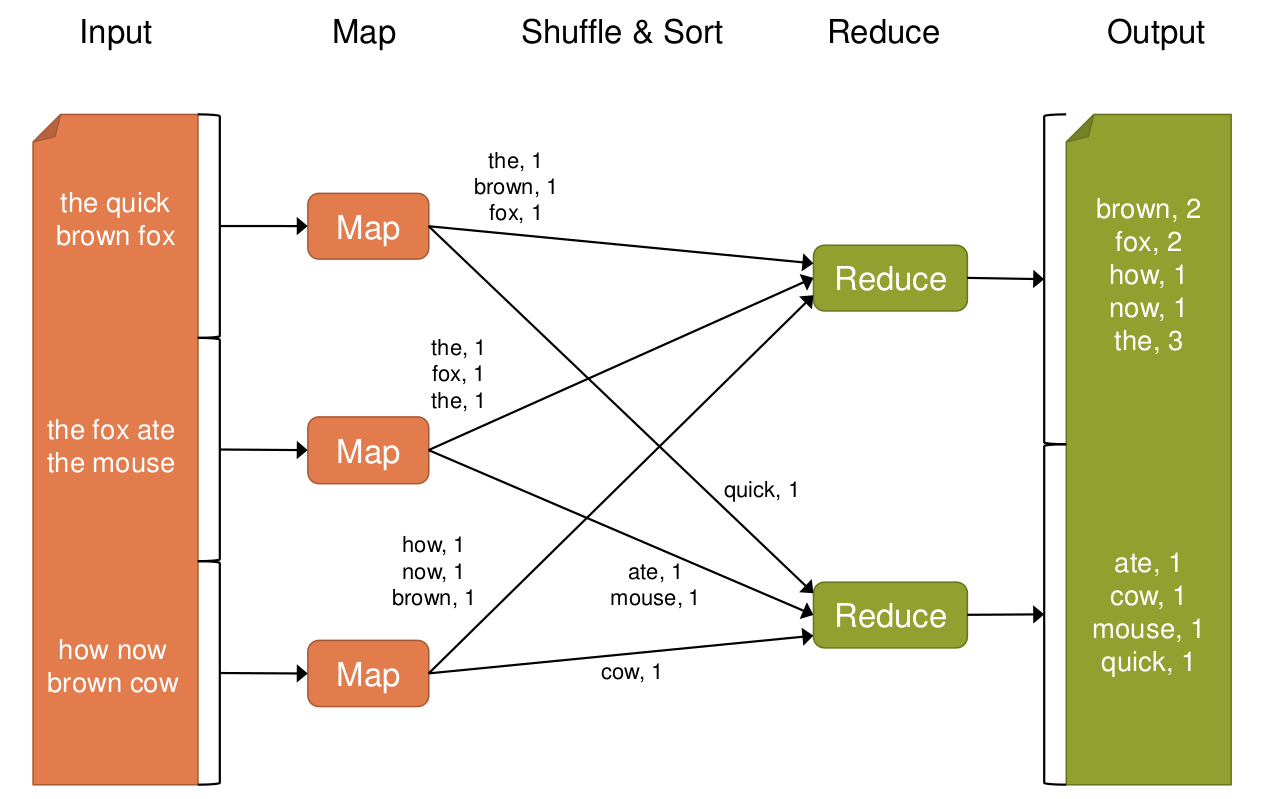
\includegraphics[width=.8\textwidth]{images/map_reduce_example.png}
  \caption{MapReduce for Word Count}\label{fig:map_reduce_example}
\end{figure}

\subsection{Message-oriented Architectures}
\subsubsection{Message-oriented Middleware (MOM)}
For MOM client and service providers look alike, the difference is only conceptual.
Messages are structured data defined by a type and consisting of name-value pairs clients and service providers have to agree on.\\
They can either be \textbf{command messages} which tell the receiver what code to run, \textbf{document messages} which transmit data or \textbf{event messages} notifying the receiver of a change in the sender.\\
MOM use message queues for communication.
Clients place messages in a queue which are typically identified by name and might be bound to intended recipients.
Whenever the recipient is ready to process a new message, it invokes the corresponding MOM function and retrieves the first message in the queue.
A \textbf{point-to-point pattern} ensures that only one receiver consumes these messages whereas a \textbf{publish-subscribe} pattern supports multiple receivers.
One should use different queues for different data types (\textbf{datatype pattern}).
\textbf{Sharded queues} can be used to distribute load among multiple applications that provide the same service.
The MOM then ensures that the message is only sent to one application.\\
\begin{minipage}[t]{0.49\textwidth}
  \textbf{Pros}
  \begin{itemize}[topsep=0pt,noitemsep]
    \item Remote communication
    \item Decoupling of systems
    \item Platform/application integration
    \item Asynchronous communication protocol (send-and-forget)
    \item Solves the issue of throttling (thanks to message queues)
  \end{itemize}
\end{minipage}
\begin{minipage}[t]{0.49\textwidth}
  \textbf{Cons}
  \begin{itemize}[topsep=0pt, noitemsep]
    \item Complex programming model (?)
    \item Scenarios where applications need synchronous solutions
    \item Message sequence issues (message channels do not guarantee when a message will be delivered)
  \end{itemize}
\end{minipage}
\vspace{20pt}

\subsubsection{Enterprise Application Middleware (EAM) Middleware: Message Brokers}
Message brokers act as a broker among system entities and are thereby creating a communication infrastructure for integrating applications (rather than only resource managers).
They decouple the sender and the receiver by providing a single point of communication between them.
They therefore also handle the routing between the two.
Receivers/subscribers have to subscribe to messages of a given type and will receive them as soon as the sender/publisher publishes them.
Several different services can be integrated using adapters.\\
Message brokers do have some challenges.
First, they might not scale very well with multiple connections, secondly security becomes an issue when having to handle a large amount of SSL certificates.
Furthermore monitoring and debugging becomes expensive and maintenance is impossible without affecting the clients.

\subsubsection{Reactive Systems}
Reactive applications employ an architecture that allows you to build systems that are responsive, resilient, elastic, and message-driven and that are capable of producing a real-time feel.

\paragraph{Actor Model}
In the actor model an actor can react in three different ways upon receiving a message.
Either it creates new actors, sends messages to actors it knows or designates how it should handle the next message it receives.
It is fundamentally based on exchanging data only via messages.\\
\begin{minipage}[t]{0.49\textwidth}
  \textbf{Pros}
  \begin{itemize}[topsep=0pt,noitemsep]
    \item Message-driven approach is more intuitive
    \item Directly and transparently applicable for distributed programming
    \item Type-safe systems
    \item Separation of concerns – clear distribution of responsibilities for actors
    \item Ensures loose coupling, isolation, and location transparency
  \end{itemize}
\end{minipage}
\begin{minipage}[t]{0.49\textwidth}
  \textbf{Cons}
  \begin{itemize}[topsep=0pt, noitemsep]
    \item Message-passing is slower
    \item Actors do not work well when synchronous shared-state behavior is required
    \item Steep learning curve (Scala with Akka)
  \end{itemize}
\end{minipage}
\vspace{20pt}

\subsection{Object-oriented architectures}
\textbf{Object brokers} extend the remote procedure call paradigm to the object-oriented world and provide services that simplify the development of distributed object oriented applications.
It extends RPC by inheritance and polymorphism in that the middleware binds clients to specific objects running on a server and manage their interactions.\\
The Common Object Request Broker Architecture (CORBA) specification is the best known example of such an architecture.
It offers a standardized specification of an object broker rather than an implementation.
Figure~\ref{fig:corba} shows the basic architecture of CORBA.
\begin{figure}[h]
  \centering
  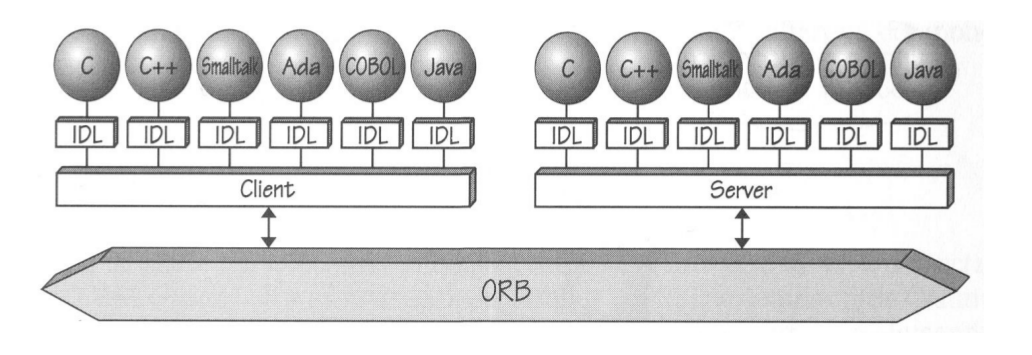
\includegraphics[width=.8\textwidth]{images/corba.png}
  \caption{CORBA}\label{fig:corba}
\end{figure}

\begin{minipage}[t]{0.45\textwidth}
  \textbf{CORBA was needed because no technology addressed all of the following requirements}
  \begin{itemize}[topsep=0pt,noitemsep]
    \item Bit protocol
    \item Open interfaces
    \item A single governance
    \item Object-orientation
    \item Language independence
    \item Operating system independence
    \item Freedom from technologies
    \item Data-typing
    \item High tunability
    \item Freedom from data-transfer details
    \item Compression
  \end{itemize}
\end{minipage}
\hspace{.05\textwidth}
\begin{minipage}[t]{0.45\textwidth}
  \textbf{CORBA in practice had a set of drawbacks that ultimately lead to low adoption for business applications:}
  \begin{itemize}[topsep=0pt, noitemsep]
    \item No standard tools
    \item Hard to deploy
    \item Heavy weight
    \item Complex toolchain
    \item Initial implementation incompatibilities
    \item Location transparency
    \item Design and process deficiencies
    \item Problems with implementations
    \item Firewall incompatibilities
  \end{itemize}
\end{minipage}
\vspace{20pt}

\subsection{Component-based Architectures}
\subsubsection{Java EE}
Java EE has a multi-tier architecture as shown in Figure~\ref{fig:java_ee}
\begin{figure}[h]
  \centering
  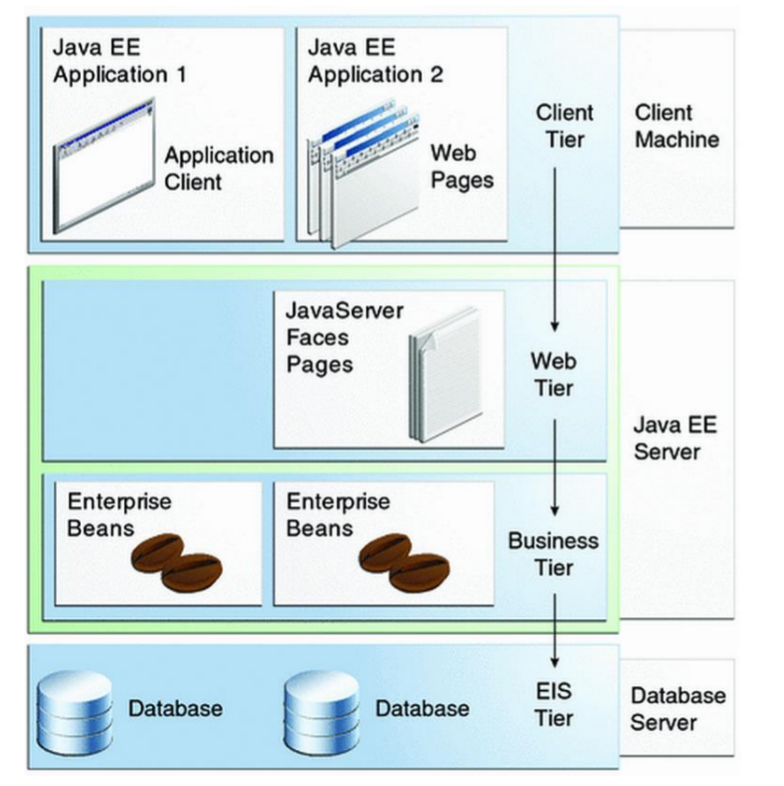
\includegraphics[width=.6\textwidth]{images/java_ee.png}
  \caption{Java EE Architecture}\label{fig:java_ee}
\end{figure}
The client tier are the (remote) applications that access the JEE server.
The web tier manages interaction between client and business tier like content generation and session management.
The business tier realizes the business logic and the enterprise information system tier consists of databases, ERP systems, data warehoses and such.\\

\paragraph{Application Server}
The \textbf{application server} mediates access to system resources, handles life-cycle, deployment, communication and security management and is encapsulated into containers.
The application client container manages application client components, the EJB (enterprise java beans) container the Java Beans components and the web container the JSP and servlet components.\\

\paragraph{Enterprise Java Beans (EJB)}
EJBs realize the business logic and can be of three different types.
Session beans are generally available for one session and are used for only one client.
They can be stateless so that they represent a state for only one method invokation, stateful for maintaining a state and singleton (somewhat exceptional?) for only one instance per server and shared among clients.
Message-driven beans are used for asynchronous processing of messages.
The last kind of beans are entity beans, but they are deprecated since J2EE 1.4.\\
Clients are able to access enterprise via a no-interface view where the beans expose the public methods of the EJB implementation to clients or with the help of a business interface (annotated with @Local and @Remote).
Receiving them is done either via dependency injection (@EJB) or with a Java Naming and Directory Interface (JNDI) lookup (remote beans [java:global], local beans [java:module, java:app]).

\paragraph{Java Persistence API}
The Java persistence API can be used to store POJOs to relational databases.
Classes then are tables, object rows and attributes columns with the help of annotations.
The EntityManger API then is used to create or remove persistent mappings and query over entities.

\paragraph{Java Messaging Service (JMS)}
The JMS is the MOM for java which supports point-to-point as well as publish-and-subscribe topologies.
Messages consist of a header (standard attributes), properties (optional attributes) and a body (actual payload).

\paragraph{Java Web Components}
\textbf{Java Servlets} are classes that respond to client requests.
\textbf{JavaServer Pages} are text based documents which mostly consist of HTML but also include some special tags that contain java code.
\textbf{JavaServer Faces} is a MVC based web framework which uses templates (facelets) for views.

\paragraph{Deployment}
Java EE applications can either be deployed non-distributed where only one functionality layer and one database layer exist or distributed where web and application server are also separated.

\subsubsection{AUTOSAR}
AUTOSAR stands for Automotive Open System Architecture and is a standardized automotive reference architecture.
Its main focuses are modularity, scalability, portability and reusability.

\paragraph{Architecture}
The AUTOSAR architecture is shown in Figure~\ref{fig:autosar}
\begin{figure}[h]
  \centering
  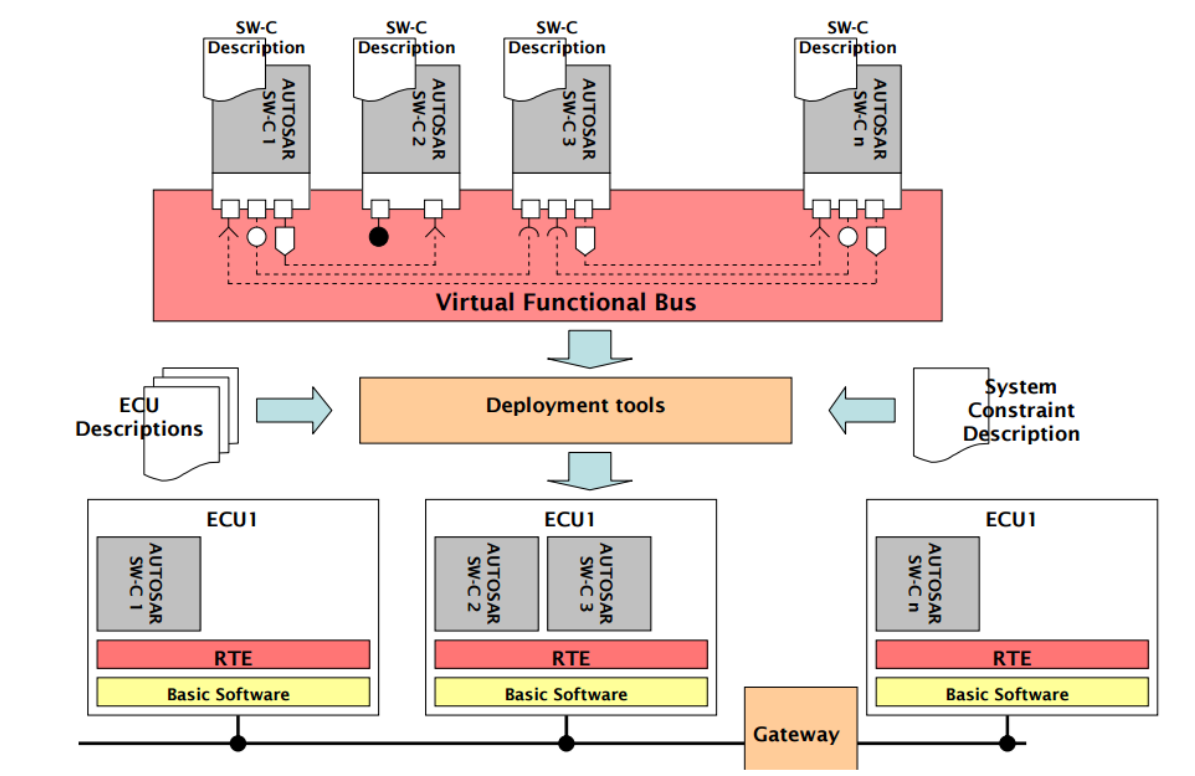
\includegraphics[width=.8\textwidth]{images/autosar.png}
  \caption{AUTOSAR Architecture}\label{fig:autosar}
\end{figure}
AUTOSAR Software Components (SW-C) encapsulate an application that runs on the AUTOSAR infrastructure for which a standard description is provided.
The Virtual Functional Bus (VFB) is an abstract representation of all communication mechanisms available.
To integrate SW-Cs into a network of ECUs, AUTOSAR provides description formats for the system as well as for the resources and configurations of ECUs.
The Runtime Environment (RTE) provides a common platform for SW-Cs.
To establish that environment on ECUs, the methodology and tool support is provided by AUTOSAR.\\

Regarding a module/ECU, there are four layers.
The application layer consists of the applications developed against the RTE that realize functionality of sensors and actuators.
The AUTOSAR RTE layer defines interfaces and basic library functions for the application layer and is the bridge to the basic software layer.
This then is the actual operating system that handles things like memory management and communication.
The lowest layer is the microcontroller abstraction layer which provides an abstraction from the I/O and communication with the microcontroller.\\

AUTOSAR communication is routed via the RTE and can be done in two different paradigms.
Either in client/server mode which is a two-way communication method or in sender/receiver mode which is a publish-and-subscribe style.\\

When deploying, all nodes have an AUTOSAR infrastructure and SW-C will be deployed at their corresponding ECUs.
That lets them communicate via the VFB which either handles messages via the RTE (intra-ECU) or physical buses (inter-ECU).
